\documentclass[conference]{IEEEtran}
%\IEEEoverridecommandlockouts
% The preceding line is only needed to identify funding in the first footnote. If that is unneeded, please comment it out.

\usepackage{graphicx}
\usepackage{subcaption}


\usepackage{cite}
\usepackage{amsmath,amssymb,amsfonts}
\usepackage{algorithmic}
\usepackage{graphicx}
\usepackage{textcomp}
\usepackage{xcolor}
\usepackage{hyperref}

\captionsetup{
  font={footnotesize} % Set the font size for all captions to 8pt (footnotesize)
}




\def\BibTeX{{\rm B\kern-.05em{\sc i\kern-.025em b}\kern-.08em
    T\kern-.1667em\lower.7ex\hbox{E}\kern-.125emX}}

\begin{document}

\title{EC Number Prediction Using Pre-Trained Language Models: A Promising Tool for Protein Research}

\author{\IEEEauthorblockN{Ugur Dura\IEEEauthorrefmark{1}}
\IEEEauthorblockA{\textit{Informatics Department} \\
\textit{Technical University of Munich}\\
Munich, Germany \\
ugur.dura@tum.de}
}

\maketitle

\begin{abstract}
Enzyme Commission (EC) numbers play a vital role in accurately understanding enzyme functions and their impact on cellular metabolism. In this paper, we explore the potential of utilizing pre-trained language models for EC number prediction, with a specific focus on protein sequences as a rich source of information. Our objective is to leverage deep learning models, particularly the transformer BERT model, to uncover patterns corresponding to the topological sites of each enzyme that may lead to predict their functionalities. Through comprehensive experimentation, we demonstrate the successful utilization of the transformer BERT model for identifying and classifying de novo enzyme functions based on protein sequences retrieved from UniProt. By treating proteins as linguistic entities, we harness the power of language models to enhance EC number prediction with a high level of accuracy. While our results showcase the effectiveness of this approach, further research is required to improve the classification accuracy for all four digits of the EC number. Future work will focus on refining the training process and incorporating additional contextual information to further enhance the model's performance. In conclusion, our study presents a promising tool for EC number prediction using pre-trained language models. By bridging the gap between protein sequences and language processing, this approach opens up new possibilities for advancements in protein research, including drug discovery, protein engineering, and biomedical applications.
\end{abstract}

\begin{IEEEkeywords}
component, formatting, style, styling, insert
\end{IEEEkeywords}

\section{Introduction}


Enzymes, a vital class of proteins within the human body, play a crucial role in catalyzing reactions and regulating various biological processes \cite{1}. Understanding their functions is essential for numerous applications, such as metagenomics, industrial biotechnology, and diagnosing enzyme-related diseases \cite{2}. However, traditional experimental techniques like enzymatic assays have become increasingly time-consuming and challenging to keep up with the rapidly growing number of newly discovered enzymes \cite{3}.

In recent years, computational methods have emerged as invaluable tools for predicting enzyme function and guiding experimental validation. The widely used Enzyme Commission (EC) system employs four-digit codes to specify enzyme functions, enabling computational methods to accurately annotate enzyme activities \cite{4}.

To address this issue, computational methods have emerged as valuable tools for predicting enzyme function and guiding experimental validation. Previous research \cite{5} has explored three main approaches for enzyme EC number prediction: (i) structure-based prediction \cite{6},\cite{7},\cite{8}, which involves first predicting enzyme structures and then assigning EC numbers based on similarities to known templates; (ii) sequence similarity-based methods\cite{9},\cite{10},\cite{11}, which predict enzyme function based on the assumption that enzymes with high sequence similarity tend to have similar functionalities; and (iii) machine learning-based methods\cite{12},\cite{13},\cite{14}, which extract features from enzyme sequences and use machine learning algorithms for classification.

Despite progress made, existing approaches encounter challenges such as homology requirements, feature design limitations, and feature dimensionality non-uniformity\cite{5},\cite{14}. Homology requirements can limit the prediction capability of sequence similarity-based methods when encountering sequences with limited homologies in existing databases\cite{15}. Moreover, feature design often relies on manually crafted or pre-defined features, which may not be optimal or sustainable in the omic era, with the rapid expansion of known enzyme sequences\cite{3},\cite{5}.

In contrast, recent advances in deep neural networks have shown promise as generative and discriminative models for protein science and engineering\cite{16}. Transformer-based language models, particularly, have demonstrated impressive capabilities in various domains, including natural language processing\cite{17}. To address these challenges, this research proposes a novel approach based on deep learning, specifically utilizing Prot-BERT\cite{18} and transfer learning, for predicting first-order EC numbers of enzymes.

In conclusion, this research aims to develop a robust and efficient deep learning-based predictive model for enzyme EC number classification. By combining the power of Prot-BERT with fine-tuning on a large dataset of enzyme sequences, this approach holds the potential to significantly advance our understanding of enzyme functions and aid in various applications related to enzymology.

\newpage


\section{Materials and Methods}\label{sec11}

\subsection{Data Collection}

The dataset used in this study was obtained from SwissProt, a manually curated section of UniProtKB, which contains a vast collection of annotated protein entries\cite{19}. Initially, the dataset comprised 565,254 protein sequences. To focus specifically on enzymes and their respective functions, a rigorous filtering process was applied, resulting in a refined dataset consisting of 271,464 entries. Only entries with at least one assigned EC number were retained for further analysis. In cases where an entry contained multiple EC numbers, the first one listed was used for subsequent prediction tasks.



\subsection{Data Analysis and Preprocessing}



To prepare our dataset for the deep learning model, we considered amino acids as the fundamental building blocks, much like an alphabet, used to train the Masked Language Model (MLM). Each amino acid was denoted by a shorthand one-letter symbol, such as 'M' for methionine, 'R' for arginine, and 'X' for unknown amino acids. This concise representation enabled us to effectively handle the diverse range of amino acid sequences present in the dataset. The distribution of amino acid letters in the dataset can be seen in Fig. \ref{fig:dataset_analysis}. Notably, leucine emerged as the most common amino acid, and our dataset did not contain any unknown amino acids.



\begin{figure}[htp!]
  \centering
  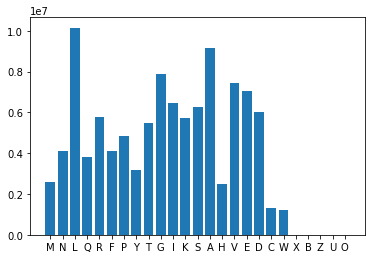
\includegraphics[width=0.8\linewidth]{images/UniqueAminoAcids.png}
  \caption{The plot illustrates the amino acid letter density distribution within the collected dataset. The y-axis represents the number of occurrences, while the x-axis displays the corresponding amino acid letters.}
  \label{fig:dataset_analysis}
\end{figure}





\begin{figure}[htp!]
  \centering
  \begin{subfigure}[b]{1\linewidth}
      \centering
    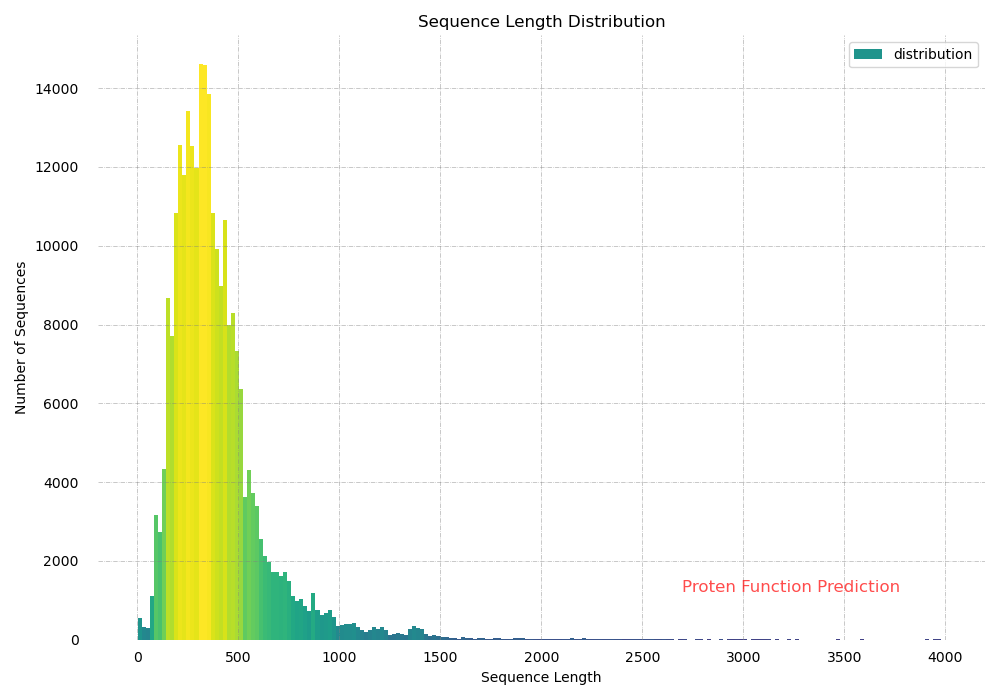
\includegraphics[width=1\linewidth]{images/Sequence_SizeDistribution(2000).png}
    \caption{}
    \label{fig:subfig1}
  \end{subfigure}
  \vspace{0.5cm} % Adjust the vertical space between subfigures
  \begin{subfigure}[b]{1\linewidth}
      \centering
    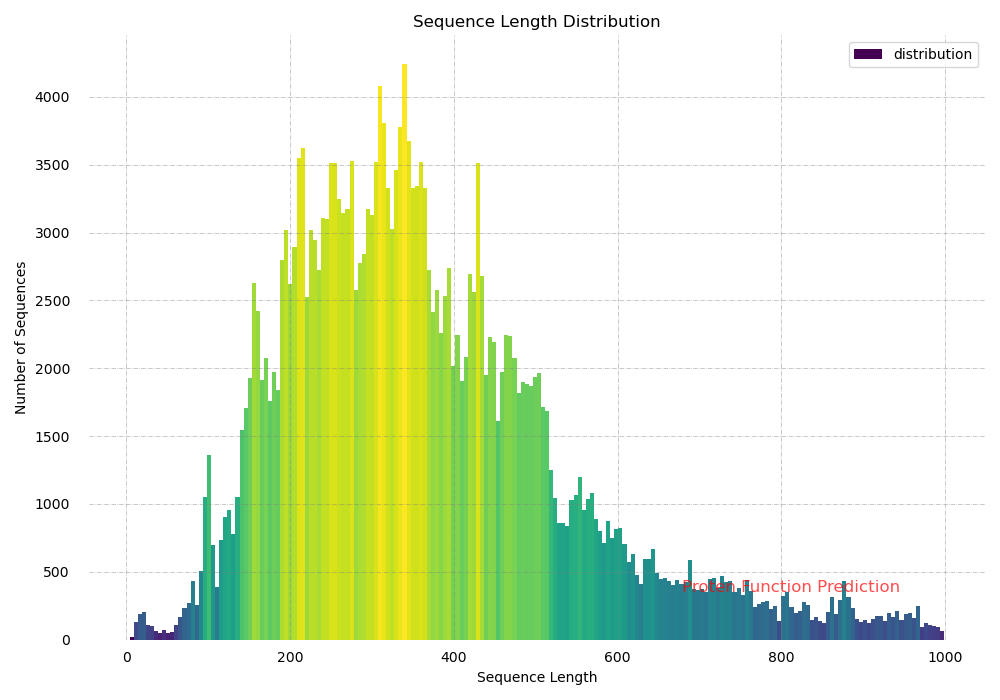
\includegraphics[width=1\linewidth]{images/Sequence_SizeDistribution(1000).png}
    \caption{}
    \label{fig:subfig2}
  \end{subfigure}
  \caption{The sequence length histogram of the dataset. The X-axis shows the sequence length and the Y-axis shows the number of sequences accumulated within that range. Left: Sequence length distribution histogram on the whole dataset. Right: Sequence length distribution histogram with range 0-1000.}
  \label{fig:Sequence_SizeDistribution}
\end{figure}





During the data analysis process, one crucial aspect that needed consideration was the variation in sequence lengths. To tokenize and train our model effectively, we needed to decide on a fixed array size for the sequences. Our analysis revealed a significant distribution of sequence lengths, with the majority falling within the range of 200 to 500 amino acids as shown in Fig. \ref*{fig:Sequence_SizeDistribution}. This finding presented a challenge, as we had to strike a balance between capturing relevant information and computational efficiency(Fig. \ref*{fig:Padding_Truncation}). Ultimately, an array size of 512 was chosen to accommodate the majority of sequences within this length range.



\begin{figure}[htp!]
  \centering
  \begin{subfigure}[b]{0.8\linewidth}
      \centering
    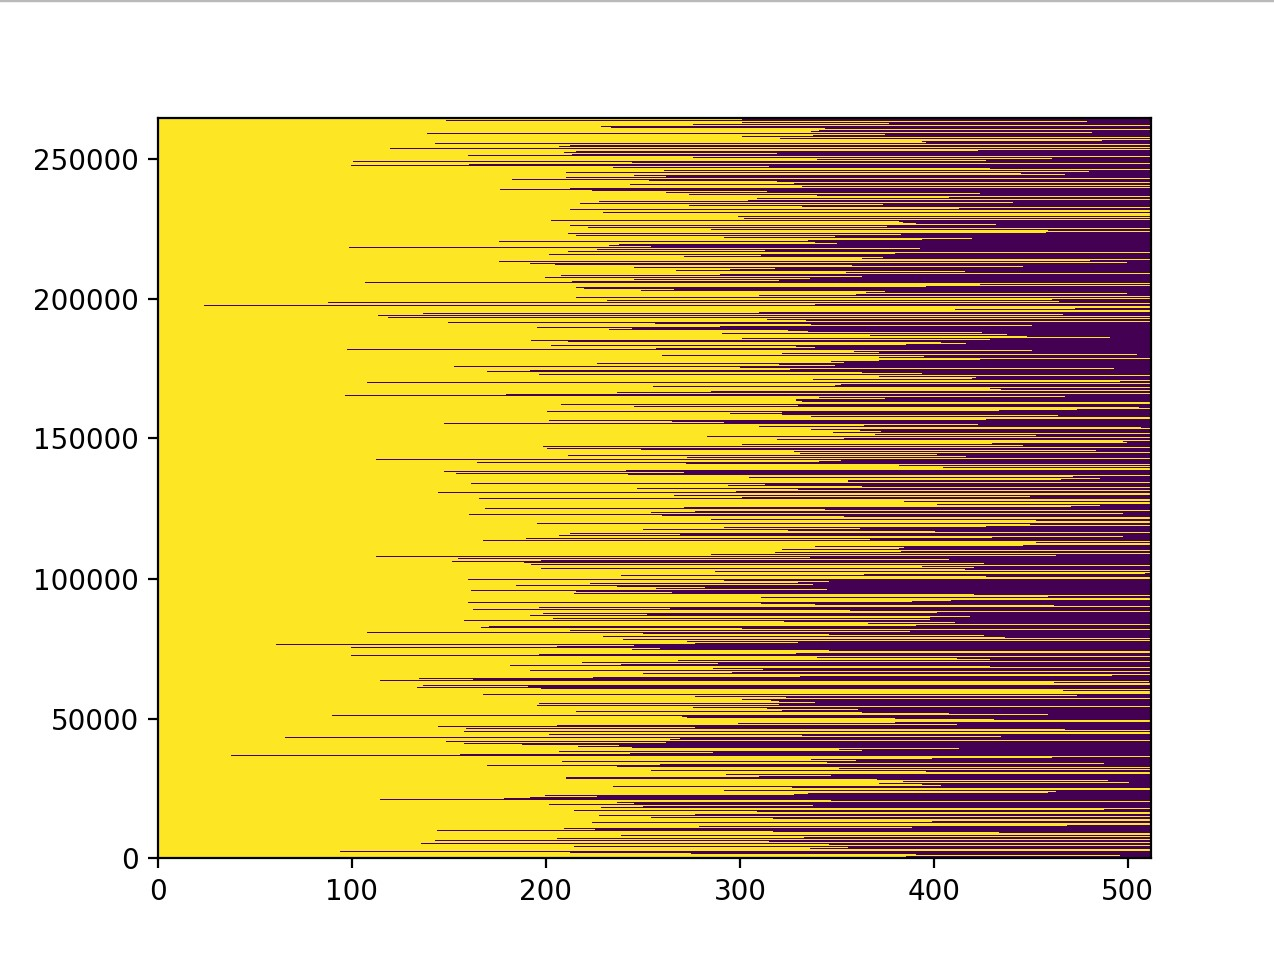
\includegraphics[width=0.8\linewidth]{images/XMASK_Padding_Truncation_Distribution.jpg}
    \caption{}
    \label{fig:subfig1}
  \end{subfigure}
  \vspace{0.5cm} % Adjust the vertical space between subfigures
  \begin{subfigure}[b]{0.8\linewidth}
      \centering
    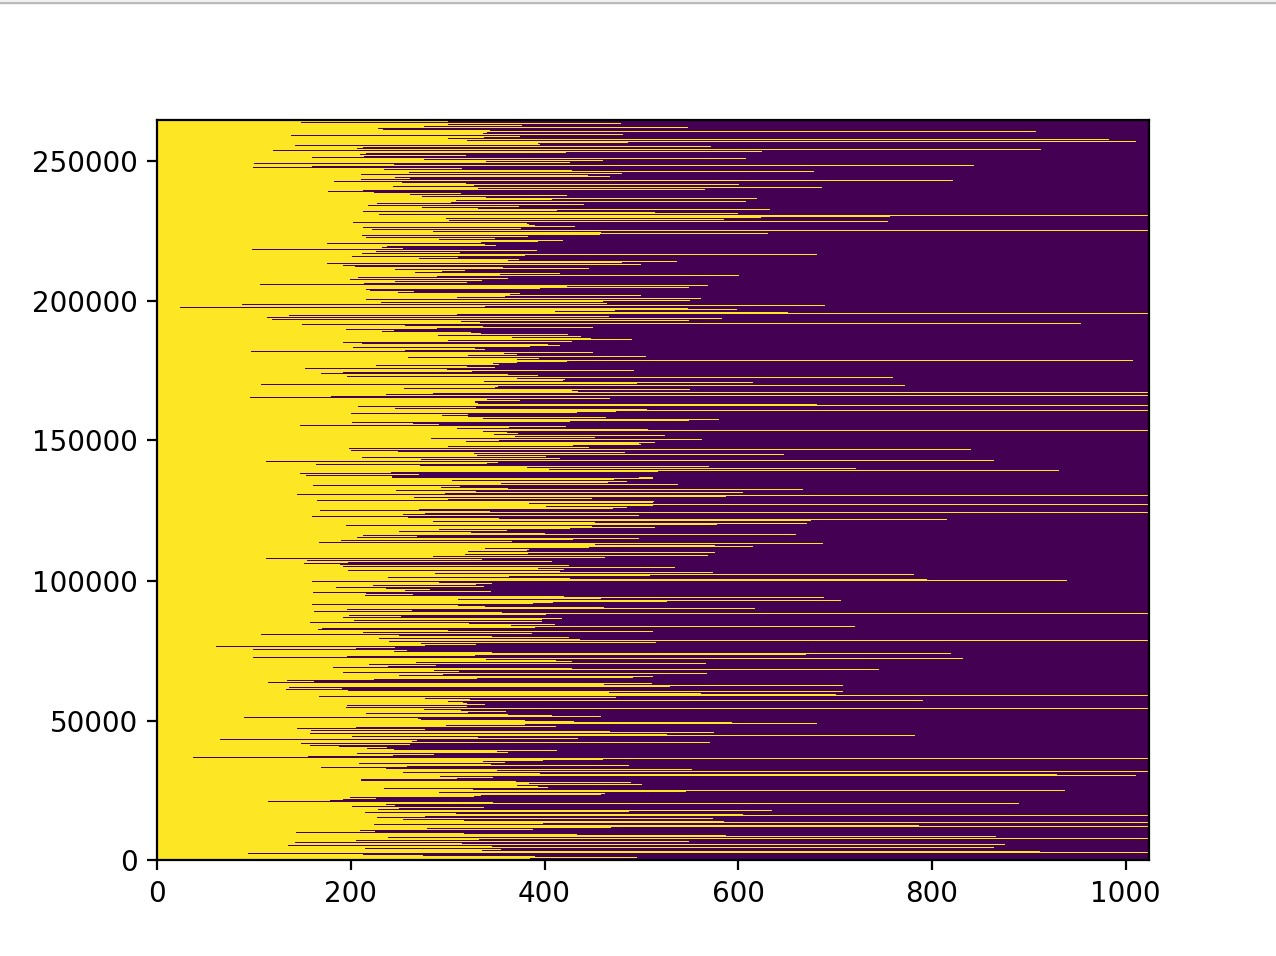
\includegraphics[width=0.8\linewidth]{images/XMASK_Padding_Truncation_Distribution_1024.jpg}
    \caption{}
    \label{fig:subfig2}
  \end{subfigure}
  \caption{Representation of the padding and truncation rate of the sequence during tokenization. The X-axis represents the length of the sequence ( for (a) max length=512, for (b) max length= 1024), the Y-axis represents the data-set index(262K entry). Yellow shows the tokenized sequence and purple shows the padded area.}
  \label{fig:Padding_Truncation}
\end{figure}



At the end of this data preprocessing, we employed one-hot encoding to effectively serve the amino acid sequences into our deep learning model. One-hot encoding is a technique that converts categorical data, such as the shorthand one-letter symbols representing amino acids, into binary vectors. Each amino acid symbol was transformed into a binary vector of zeros and ones, with a value of one at the position corresponding to the specific amino acid and zeros elsewhere. Let A be a set containing specific amino acid letters, and $\mathbb{R}_A(x)$ be the indicator function. For each amino acid x, $\mathbb{R}_A(x)$ returns 1 if x is in the set A, and 0 if x is not in the set A (eq. \ref*{eq:indicator_function}).This encoding allowed the model to process the amino acid sequences as numerical inputs, facilitating the training and prediction processes.


\begin{subequations}
  \label{eq:indicator_function}
  \begin{equation}
  A = \left \{ a_1, a_2, a_3, \ldots, 21 \right \}
  \end{equation}
  
  \begin{equation}
  \mathbb{R}_A(x) =
  \begin{cases}
  1 & \text{if } x \in A, \\
  0 & \text{if } x \notin A.
  \end{cases}
  \end{equation}
  \end{subequations}



By utilizing one-hot encoding, we successfully converted the diverse range of amino acid representations in the dataset into a format suitable for input to the Masked Language Model. By understanding the characteristics of our dataset,  we were able to lay a strong foundation for the subsequent development and fine-tuning of our deep learning model. 



\subsection{Model Construction}


In our research, we utilized the main Bert Layer from the pre-trained ProtBERT-BFD\cite{18}
model as the embedding layer. The ”training” parameter of the layer was set to False
during fine-tuning to maintain the integrity of the pre-trained embedding mechanism. We
employed the mandatory ProtBERT-BFD tokenizer to tokenize our dataset. Following
the embedding layer, we used pooling, normalization, two dense layers (with sizes 128
and 32), a dropout layer, and a final dense layer with softmax activation function (Fig. \ref{fig:model}). The
tokenizer outputs, including the tokenized sequence and mask, were fed into the BERT
layer. The model’s output went through subsequent layers until the final output layer,
which provided probability scores for each class. ReLU activation function was used for
hidden layers to prevent the vanishing gradient problem and enhance model performance.


\begin{figure}[htp!]
  \centering
  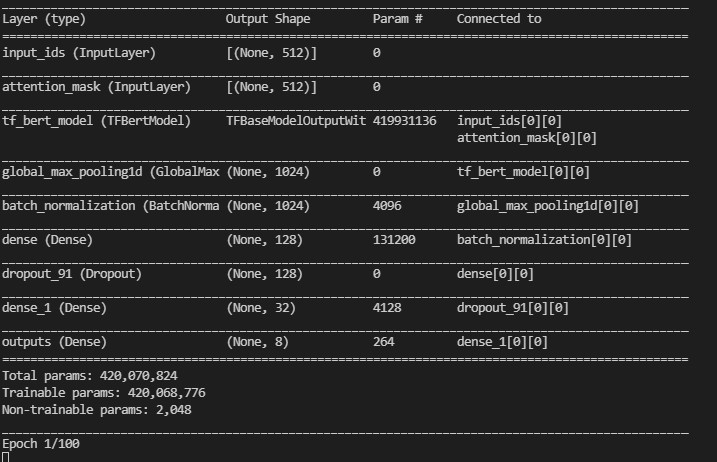
\includegraphics[width=1\linewidth]{images/Model_0001.jpg}
  \caption{Enzyme Commission number prediction up to two digits model.Hyperparameters for this model: Dataset size:
  50.000, Batch size: 32, Input array size: 512, Label array size: 72, epoch number: 10, optimizer:
  Adam, learning rate: 0.01, training and test split size: 1:9, activation function: sigmoid, output layer
  activation function: sigmoid.}
  \label{fig:model}
\end{figure}





\section{Results}

\subsection{Results of first-order EC number prediction}

Upon completing the training of our model, we conducted an assessment of various
metrics including loss, accuracy, validation accuracy, and validation loss Fig. \ref{fig:results} demonstrates a continuous decrease in loss and an increase in accuracy, indicating that our
model did not suffer from overfitting and the training process was successful.

Additionally, following the model’s successful training, we performed several tests by
loading data and predicting sequences provided by the user. The outcomes of these tests
confirmed that our model possesses the capability to accurately predict EC numbers for
the requested sequences.

\subsection{Results of second, third and fourth-order EC number prediction}

We extended our predictions to include second, third, and fourth orders of the EC number
to obtain more specific information about the enzymes. As the order of the EC number
increased, the number of classes (labels) also increased. For example, the second order
had 72 classes, the third order had 207 classes, and the fourth order had 272 distinct
classes. Due to the increasing complexity of the EC numbers, predicting the exact EC
number based on a limited dataset became more challenging. However, we made every
effort to achieve the best possible results, as shown in Fig. \ref{fig:results}.

\onecolumn


\begin{figure}[ht]
  \centering

  \begin{subfigure}{0.7\linewidth}
    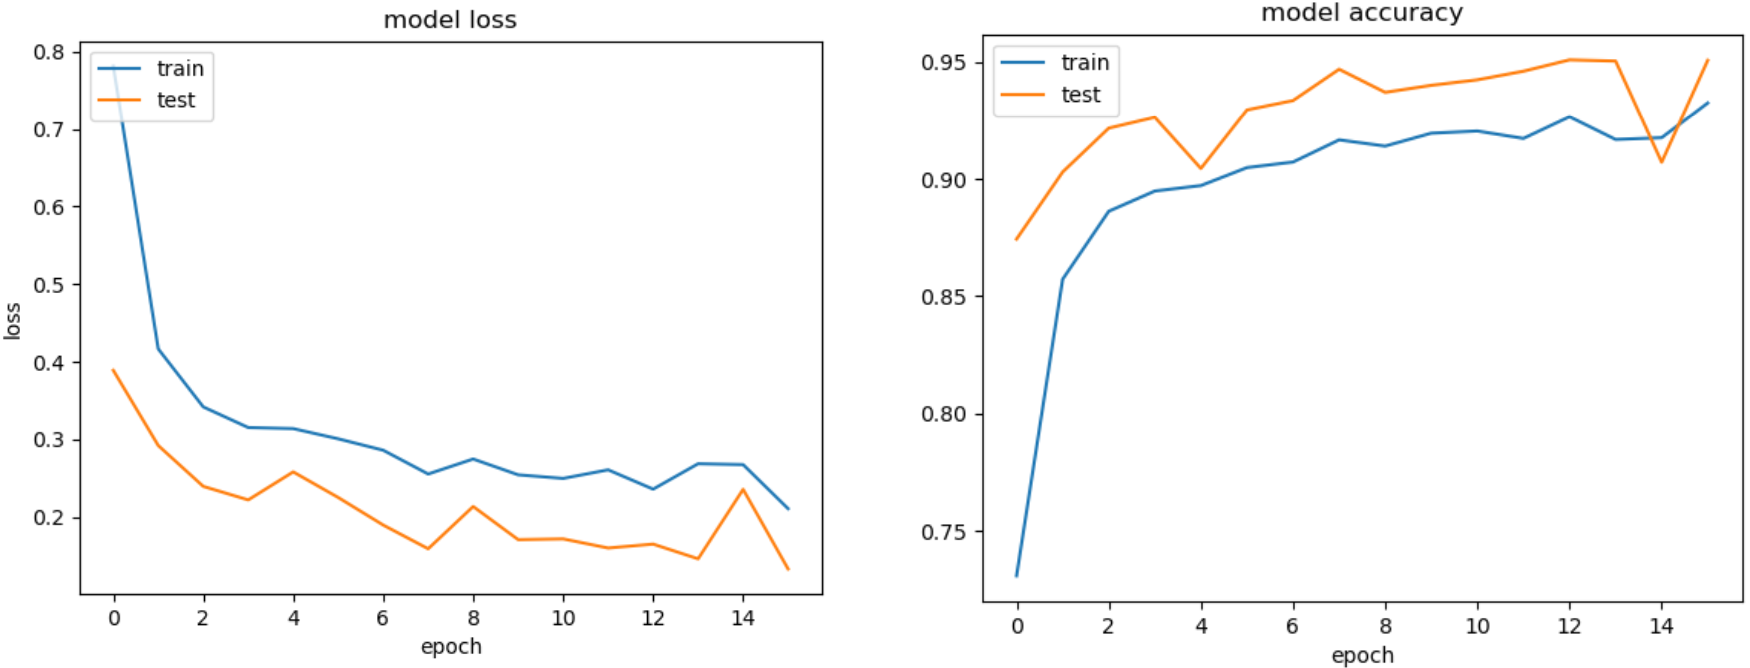
\includegraphics[width=\linewidth]{images/EC1_Results.png}
    \caption{First-order EC number predictions}
    \label{fig:subfig1}
  \end{subfigure}

  \vspace{0.5cm}

  \begin{subfigure}{0.7\linewidth}
    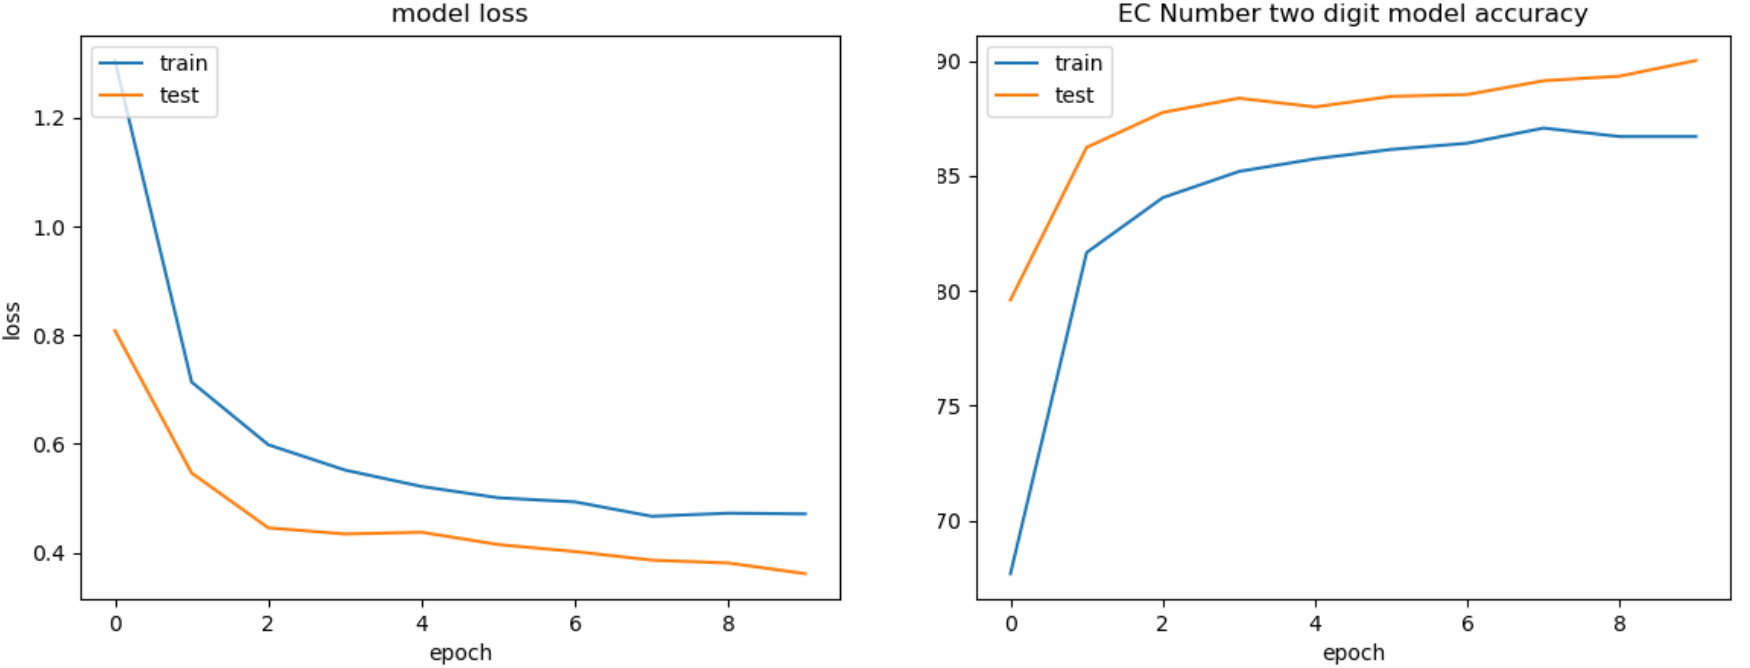
\includegraphics[width=\linewidth]{images/EC2_Results.png}
    \caption{First two digits EC number predictions}
    \label{fig:subfig2}
  \end{subfigure}

  \vspace{0.5cm}

  \begin{subfigure}{0.7\linewidth}
    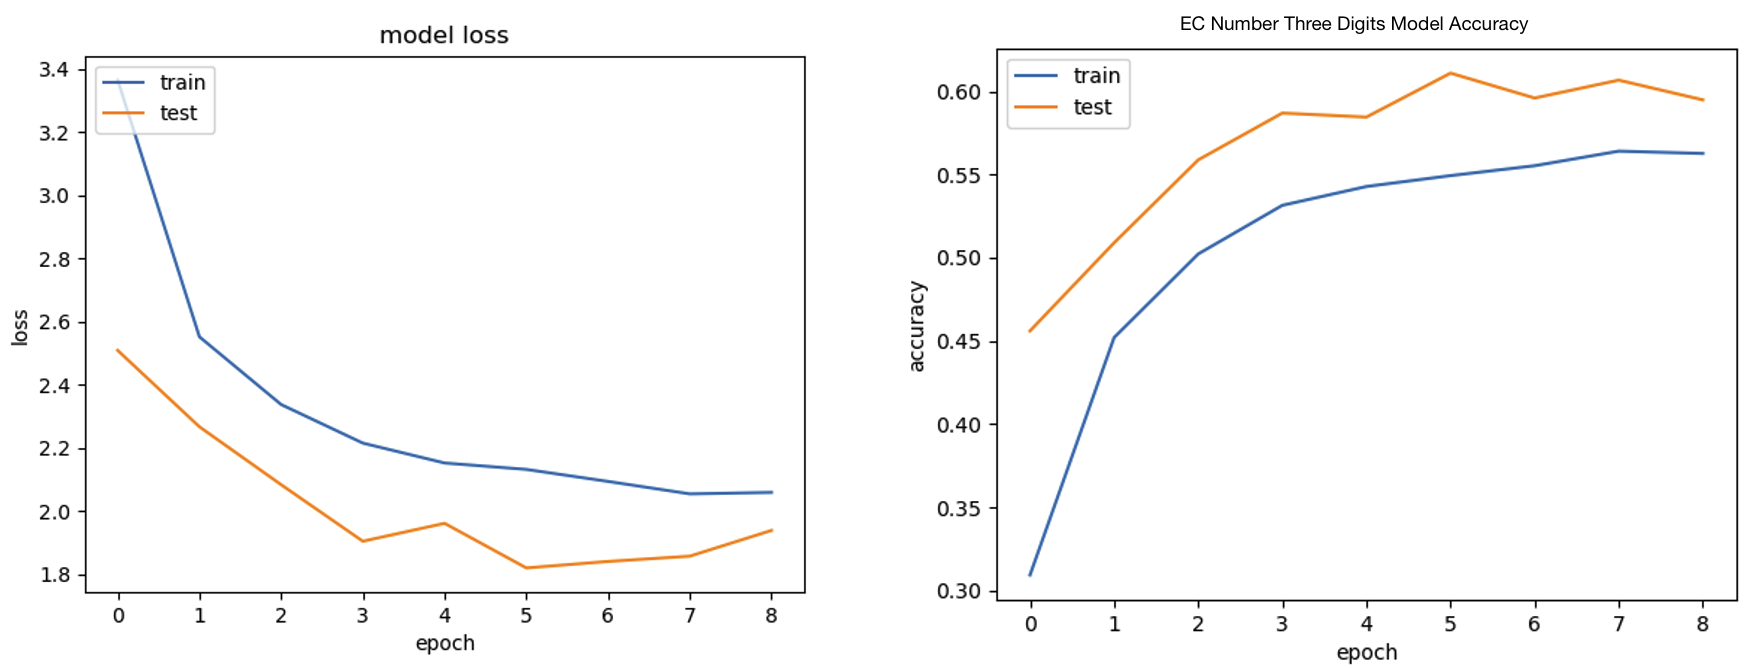
\includegraphics[width=\linewidth]{images/EC_3.png}
    \caption{First three digits EC number predictions}
    \label{fig:subfig3}
  \end{subfigure}

  \vspace{0.5cm}

  \begin{subfigure}{0.7\linewidth}
    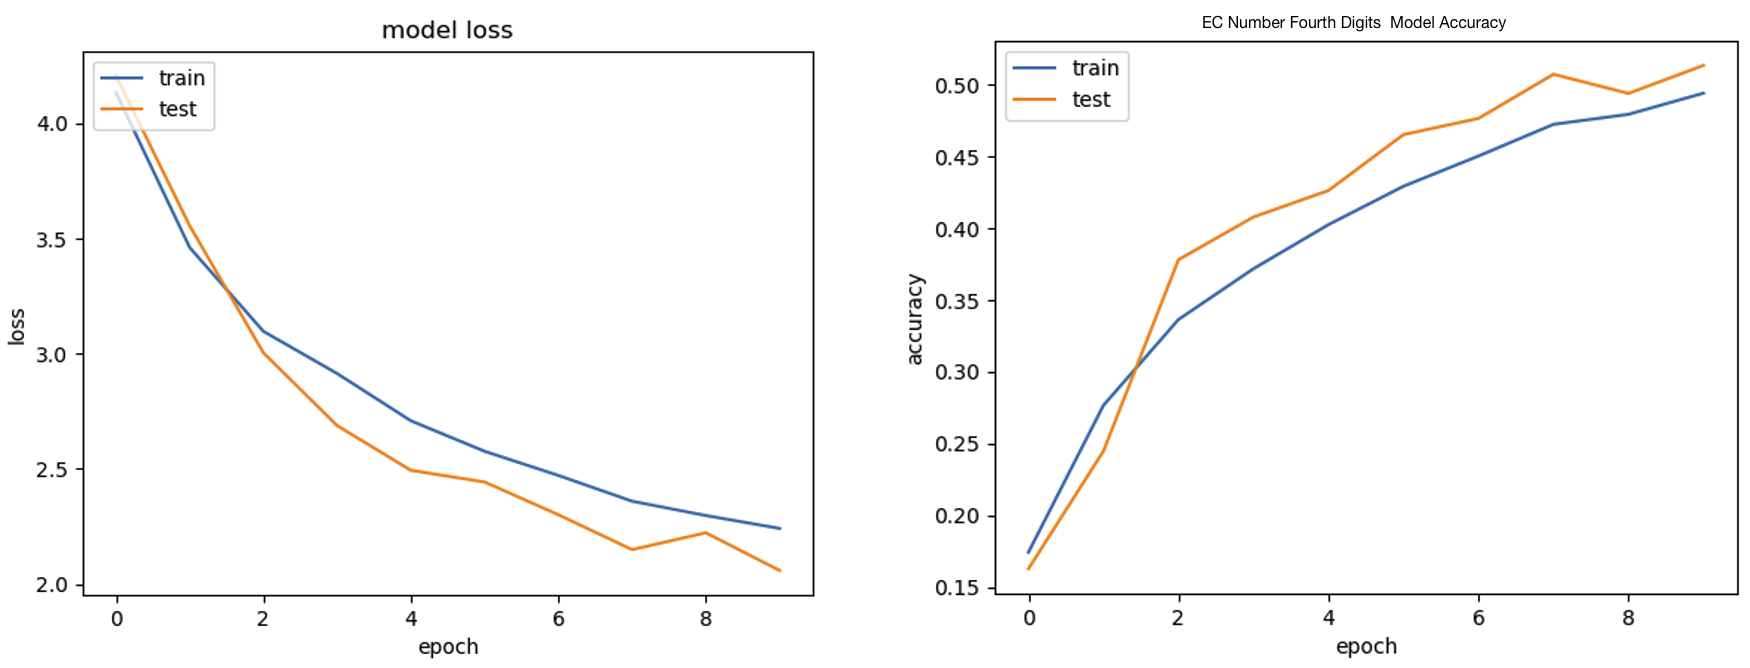
\includegraphics[width=\linewidth]{images/EC4_Results.png}
    \caption{Overall EC number predictions}
    \label{fig:subfig4}
  \end{subfigure}

  \caption{The figure displays four subplots representing the results of each model for predicting Enzyme Commission (EC) numbers. (a) illustrates the first-order EC number predictions achieved by Model 1, while the second subplot (b) shows the first two digits EC number predictions obtained by Model 2. The (c) exhibits the first three digits EC number predictions by Model 3, and the (d) demonstrates the overall EC number predictions by Model 4. Additionally, each subplot shows the model loss throughout epochs on the left side and the model accuracy throughout epochs on the right side.}
  \label{fig:results}
\end{figure}


\twocolumn



\section{Discussion}

The study employed ProtBERT-based models for predicting EC numbers of different
orders. The first-order prediction demonstrated successful training, with decreasing loss
and increasing accuracy. The model accurately predicted EC numbers for user-provided
sequences. Moving to higher orders presented challenges due to increased complexity
and limited data. However, efforts yielded noteworthy results, as depicted in Fig. \ref{fig:results}. The
first-order prediction achieved high accuracy (0.96), while accuracy slightly decreased
for higher orders (0.87 for second order, 0.64 for third order). The fourth-order prediction encountered greater difficulties, resulting in lower accuracy (52). Despite these challenges, the model showcased its potential in providing insights into enzyme functionality. Future work should focus on expanding the dataset and exploring alternative strategies for further improving accuracy and robustness.


\subsection{Further Research}

The 4-digit EC number notation is organized in a hierarchical classification structure, resembling a tree-like schema, with the general enzyme category at the root node and the 4th-order EC number at the deepest leaves. Predicting the complete 4-digit EC number can be considered a multi-label task, depending on the specific approach used.

Contrastive learning offers several advantages over traditional supervised training methods, particularly in the context of hierarchical classification tasks. In a study conducted by Heizinger et al. in 2022, the performance of contrastive learning on real protein language models was demonstrated \cite{20}. One key advantage is its dynamic nature, allowing the model to update with new data without requiring re-training, making it well-suited for online learning scenarios. Additionally, contrastive learning enables the network to learn how to access information from an external lookup set rather than memorizing the training data, leading to improved efficiency and scalability \cite{20}. Our findings suggest that contrastive learning holds promise for improving the multi-class problem we encountered. In future work, a combination of hierarchical classification and contrastive learning could be explored to address optimization challenges and further enhance model accuracy.



\section{Conclusion}


In this study, we explored the potential of utilizing pre-trained language models, particularly the transformer BERT model, for predicting EC numbers based on protein sequences. Our objective was to bridge the gap between protein sequences and language processing, leveraging the power of deep learning to accurately predict enzyme functionalities.

Through extensive experimentation on a carefully curated dataset of enzyme sequences from UniProt, we demonstrated the successful utilization of the transformer BERT model for first-order EC number prediction with high accuracy. The model effectively harnessed the linguistic information present in protein sequences, allowing us to classify de novo enzyme functions with confidence.

While higher-order EC number prediction proved more challenging due to limited data and increased complexity, our model showed promise for gaining insights into enzyme functionality at various levels.

Overall, our research demonstrates the potential of language models in enzymology, paving the way for advancements in drug discovery, protein engineering, and biomedical applications.

Future research should focus on expanding the dataset to address data limitations and further improving model accuracy for higher-order EC number prediction. Incorporating contrastive learning techniques and exploring hierarchical classification approaches could enhance optimization and scalability, allowing the model to adapt to new data seamlessly.

Overall, our study opens up exciting possibilities for leveraging deep learning in enzyme function prediction, propelling the field towards new discoveries and applications.




\begin{thebibliography}{00}
\bibitem{1} G. M. Cooper, The central role of enzymes as biological catalysts. Sunderland, MA: Sinauer Associates, 2000.
\bibitem{2} P. K. Robinson, “Enzymes: principles and biotechnological applications,” Essays Biochem., vol. 59, no. 0, pp. 1–41, 2015.

\bibitem{3} B. Rost and C. Sander, “Bridging the protein sequence-structure gap by structure predictions,” Annu. Rev. Biophys. Biomol. Struct., vol. 25, no. 1, pp. 113–136, 1996.
\bibitem{4} Q.-N. Hu et al., “Assignment of EC numbers to enzymatic reactions with reaction difference fingerprints,” PLoS One, vol. 7, no. 12, p. e52901, 2012.
\bibitem{5} Y. Li et al., “DEEPre: sequence-based enzyme EC number prediction by deep learning,” Bioinformatics, vol. 34, no. 5, pp. 760–769, 2018.
\bibitem{6} P. D. Dobson and A. J. Doig, “Predicting enzyme class from protein structure without alignments,” J. Mol. Biol., vol. 345, no. 1, pp. 187–199, 2005.
\bibitem{7}C. Nagao, N. Nagano, and K. Mizuguchi, “Prediction of detailed enzyme functions and identification of specificity determining residues by random forests,” PLoS One, vol. 9, no. 1, p. e84623, 2014.
\bibitem{8}J. Yang, R. Yan, A. Roy, D. Xu, J. Poisson, and Y. Zhang, “The I-TASSER Suite: protein structure and function prediction,” Nat. Methods, vol. 12, no. 1, pp. 7–8, 2015.
\bibitem{9}A. K. Arakaki, Y. Huang, and J. Skolnick, “EFICAz2: enzyme function inference by a combined approach enhanced by machine learning,” BMC Bioinformatics, vol. 10, no. 1, p. 107, 2009.

\bibitem{10}S. Quester and D. Schomburg, “EnzymeDetector: an integrated enzyme function prediction tool and database,” BMC Bioinformatics, vol. 12, no. 1, p. 376, 2011.
\bibitem{11}N. Kumar and J. Skolnick, “EFICAz2.5: application of a high-precision enzyme function predictor to 396 proteomes,” Bioinformatics, vol. 28, no. 20, pp. 2687–2688, 2012.
\bibitem{12}C. Z. Cai, L. Y. Han, Z. L. Ji, X. Chen, and Y. Z. Chen, “SVM-Prot: Web-based support vector machine software for functional classification of a protein from its primary sequence,” Nucleic Acids Res., vol. 31, no. 13, pp. 3692–3697, 2003.
\bibitem{13}H.-L. Zou and X. Xiao, “Classifying multifunctional enzymes by incorporating three different models into chou’s general pseudo amino acid composition,” J. Membr. Biol., vol. 249, no. 4, pp. 551–557, 2016.
\bibitem{14}L. De Ferrari, S. Aitken, J. van Hemert, and I. Goryanin, “EnzML: multi-label prediction of enzyme classes using InterPro signatures,” BMC Bioinformatics, vol. 13, no. 1, p. 61, 2012.
\bibitem{15}H. Dai, R. Umarov, H. Kuwahara, Y. Li, L. Song, and X. Gao, “Sequence2Vec: a novel embedding approach for modeling transcription factor binding affinity landscape,” Bioinformatics, vol. 33, no. 22, pp. 3575–3583, 2017.
\bibitem{16}K. Lin, X. Quan, C. Jin, Z. Shi, and J. Yang, “An interpretable double-scale attention model for enzyme protein class prediction based on Transformer encoders and multi-scale convolutions,” Front. Genet., vol. 13, 2022.
\bibitem{17} K. S. Kalyan, A. Rajasekharan, and S. Sangeetha, “AMMUS: A survey of transformer-based pretrained models in natural language processing,” arXiv cs.CL, 2021.
\bibitem{18}A. Elnaggar et al., “ProtTrans: Towards cracking the language of life’s code through self-supervised learning,” bioRxiv, 2020.

\bibitem{19}A. Morgat et al., “Enzyme annotation in UniProtKB using Rhea,” bioRxiv, 2019.
\bibitem{20}M. Heinzinger, M. Littmann, I. Sillitoe, N. Bordin, C. Orengo, and B. Rost, “Contrastive learning on protein embeddings enlightens midnight zone,” NAR Genom. Bioinform., vol. 4, no. 2, p. lqac043, 2022.
 
\end{thebibliography}
\vspace{12pt}



\section*{Appendix}

\subsection*{A Source Code}


Please find the source code on GitHub: \href{https://github.com/UgurDURA/Protein-Active-Site-w-ML.git}{GitHub Repository}







\end{document}
